\documentclass[CJK,aspectratio=169]{beamer}  %aspectratio控制页面的宽高比,16:9充满屏幕
\usepackage{beamerthemesplit}
\usetheme{Warsaw}
\usepackage{ctex} %中文字体设置
\usepackage{subfig}
\usepackage{amssymb,amsmath,mathtools}
\usepackage{amsfonts,booktabs}
\usepackage{lmodern,textcomp}
\usepackage{color}
\usepackage{tikz}
%\usepackage[latin1]{inputenc}
\usepackage{natbib}
\usepackage{bbding}
\usepackage{multicol}
\usepackage{caption} 
\usepackage{graphicx}
\usepackage{makecell}                 % 三线表-竖线
\usepackage{booktabs}                 % 三线表-短细横线
\addtobeamertemplate{headline}{}{%
	\begin{tikzpicture}[remember picture,overlay]
		\node[anchor=north west] at (current page.north west) {
\includegraphics[height=0.75cm, height=0.75cm]{picture/lzu-logo/png/logo-white_530x160}};
\end{tikzpicture}}

\begin{document}
	
	\title{基于边缘指导的低光图像增强方法}
	\author[Gu Rui (LZU) 中期考核汇报]{顾睿\inst{1} \\
		指导老师: 王忠}
	\institute[*]{\inst{1} 信息科学与工程学院,\\
		兰州大学\\
		npukujui11@gmail.com}
	
	\newcommand{\monthname}[1][\the\month]{%
		\ifcase#1\or
		January\or February\or March\or April\or May\or June\or
		July\or August\or September\or October\or November\or December\fi}
		
	\renewcommand{\today}{\monthname[\the\month] \the\day, \the\year}
	\renewcommand{\figurename}{图}
	\renewcommand{\tablename}{表}
	\renewcommand{\refname}{References}
	\date{\today}
	
	\begin{frame}
		\titlepage
	\end{frame}
	
	\begin{frame}
		%\begin{multicols}{2}
			\small \tableofcontents
		%\end{multicols}
	\end{frame}
	
%	\begin{frame} \transblindshorizontal<1>  %百叶窗效果
%		
%		\begin{itemize}
%			\item <1> {\bf 章节4}
%			\begin{itemize}
%				\item {章节4.1}
%				\begin{itemize}
%					\item {4.1.2}
%				\end{itemize}
%			\end{itemize}
%			
%		\end{itemize}		
%	\end{frame}
	
	\section{已知问题}
	\begin{frame}
		\begin{figure}
			\centering			
			\begin{minipage}{\columnwidth}
				\setlength{\abovecaptionskip}{-0.05cm}
				\centering
				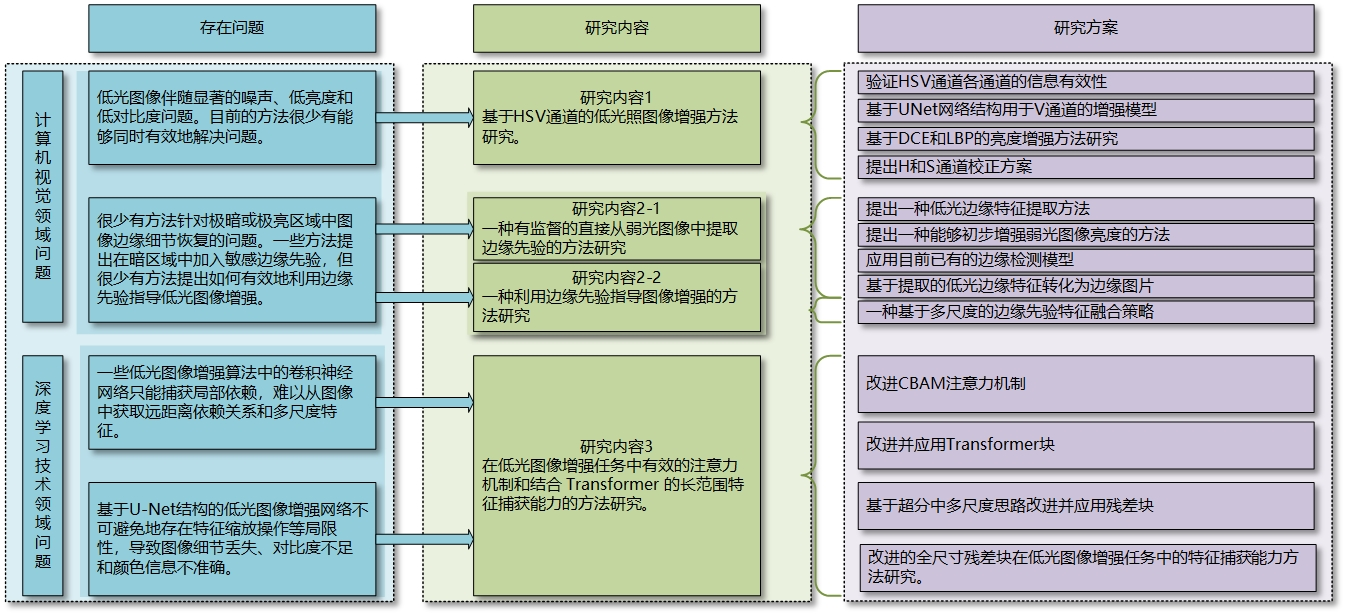
\includegraphics[width=\textwidth]{picture/LLIE/My Architecture/Total}
				%\caption{
					%	\label{fig: application scenarios}
					%	\tiny Application scenarios.
					%}
			\end{minipage}
		\end{figure}
	\end{frame}
	
	\section{模型提出}
	\begin{frame}
		\begin{figure}
			\centering			
			\begin{minipage}{.4\columnwidth}
				%\centering
				%\small
				\begin{itemize}
					\item \zihao{-5} \yahei %在弱光环境下拍摄的图像中,
					
					H 通道不仅保留了颜色信息,而且清晰地展示了颜色的变化,这些变化在此环境下可视作“颜色噪声”
					% 通过细致分析H通道,我们可以更有效地把握图像的纹理特征,并恢复出更接近真实场景的颜色表现。
					
					
					
					% 我们似乎通过综合利用色调通道提供的独特颜色识别能力,可以在不同光照条件下实现更精确的颜色复原,从而为低光图像处理提供了一种新的视角和方法论。
					\vspace{0.5cm}
					\item \zihao{-5} \yahei
					S 通道表示颜色的纯度或浓度,校正 S 通道能够恢复弱光图像的饱和度
					% S (Saturation)通道表示颜色的纯度或浓度,即色彩的深浅程度。饱和度为 0 表示灰度图像,而饱和度为 1 表示完全饱和的纯色。在某些情况下,饱和度图像可能反映出图片的一些结构信息。饱和度一般反映了像素的颜色纯度或浓度,较高的饱和度意味着颜色更加纯净和饱和,而较低的饱和度则意味着颜色更加灰暗和淡薄。在一些图像中,物体的边界或者纹理部分可能具有较高的饱和度,而背景或者平坦的区域可能具有较低的饱和度。因此,在一些情况下,饱和度图像可能会显示出物体的边界或者纹理信息。但是,并不是所有的图像都能够通过饱和度图像准确地反映出结构信息。在某些情况下,饱和度图像可能会受到光照,色彩分布和摄像机参数等因素的影响,导致其无法准确地反映出图像地结构信息。对于弱光图像来说,饱和度(S)通道通常不能很好地反映出图片地结构信息。弱光图像通常是指光照条件较差或者光照不均匀的图像,在这种情况下,图像的色彩信息可能会受到影响,导致饱和度较低,即使存在一定的色彩变化或者结构信息,也可能无法很好地体现在饱和度通道中。
					
					% V (Value)通道表示颜色的亮度或明暗程度。明度为 0 表示黑色,而明度为 1 表示白色。
					% 对于弱光图像来说,
					\vspace{0.5cm}
					\item \zihao{-5} \yahei
					V 通道通常能够更好地反映出图片的结构和纹理信息
					
					% 亮度通道代表了图像的明暗程度,而在弱光条件下,图像的色彩信息可能会受到影响,导致饱和度和色调较低,即使存在一定的色彩变化或者结构信息,也可能无法很好地体现在饱和度和色调通道中。综上所述,对于弱光图像更适合使用亮度(V)通道来反映图片的结构信息。
				\end{itemize}
			\end{minipage}
			\begin{minipage}{.5\columnwidth}
				\setlength{\abovecaptionskip}{-0.05cm}
				\centering
				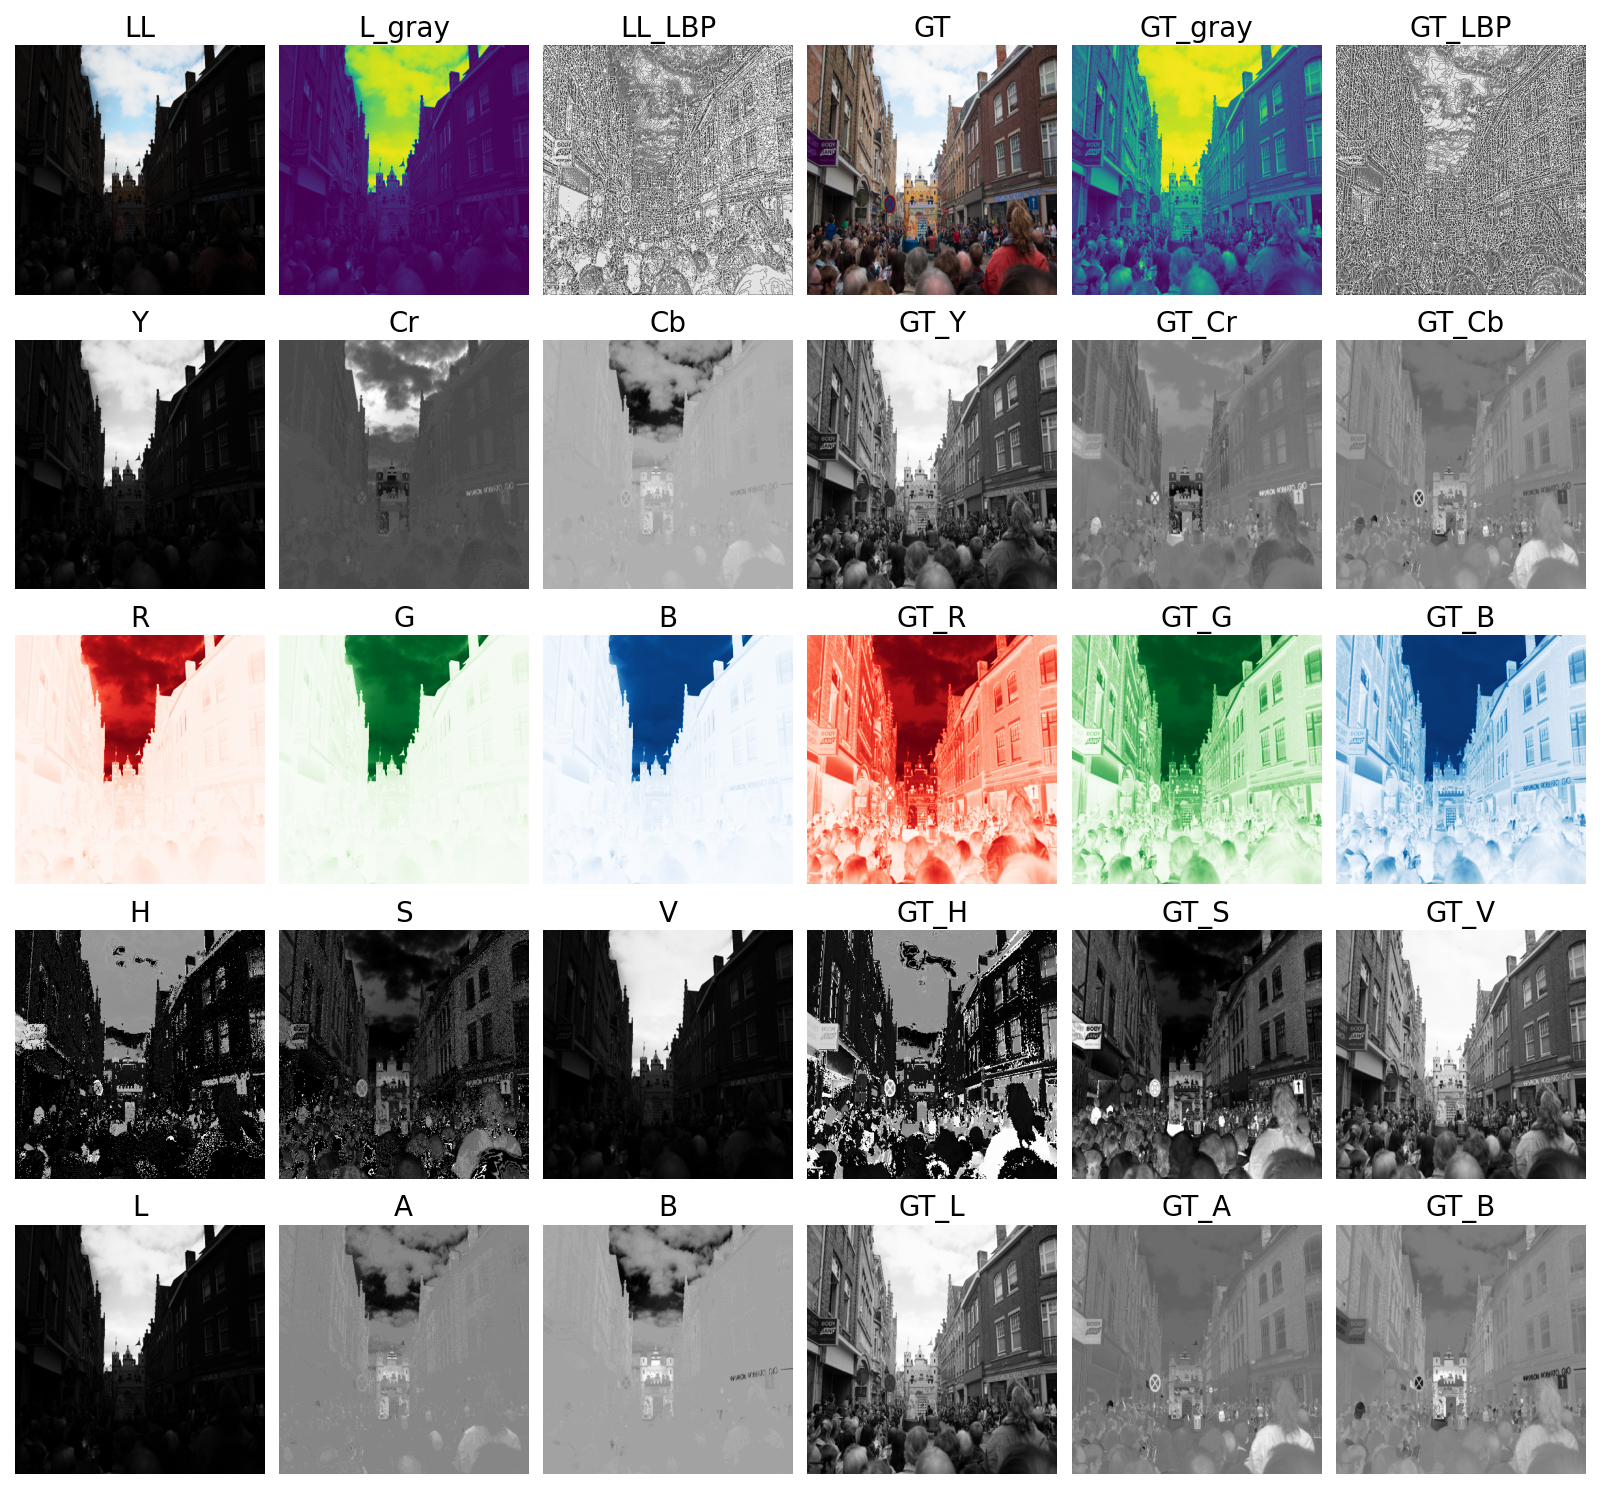
\includegraphics[width=0.9\textwidth]{picture/LLIE/Experiment/myplot_different_color_channels_r097088c1t}
				%\caption{
				%	\label{fig: application scenarios}
				%	\tiny Application scenarios.
				%}
			\end{minipage}
		\end{figure}
	\end{frame}
	
	\section{模型结构}
	
	\subsection{模型架构}
	
	\begin{frame}
		\begin{figure}[htbp]
			\begin{center}
				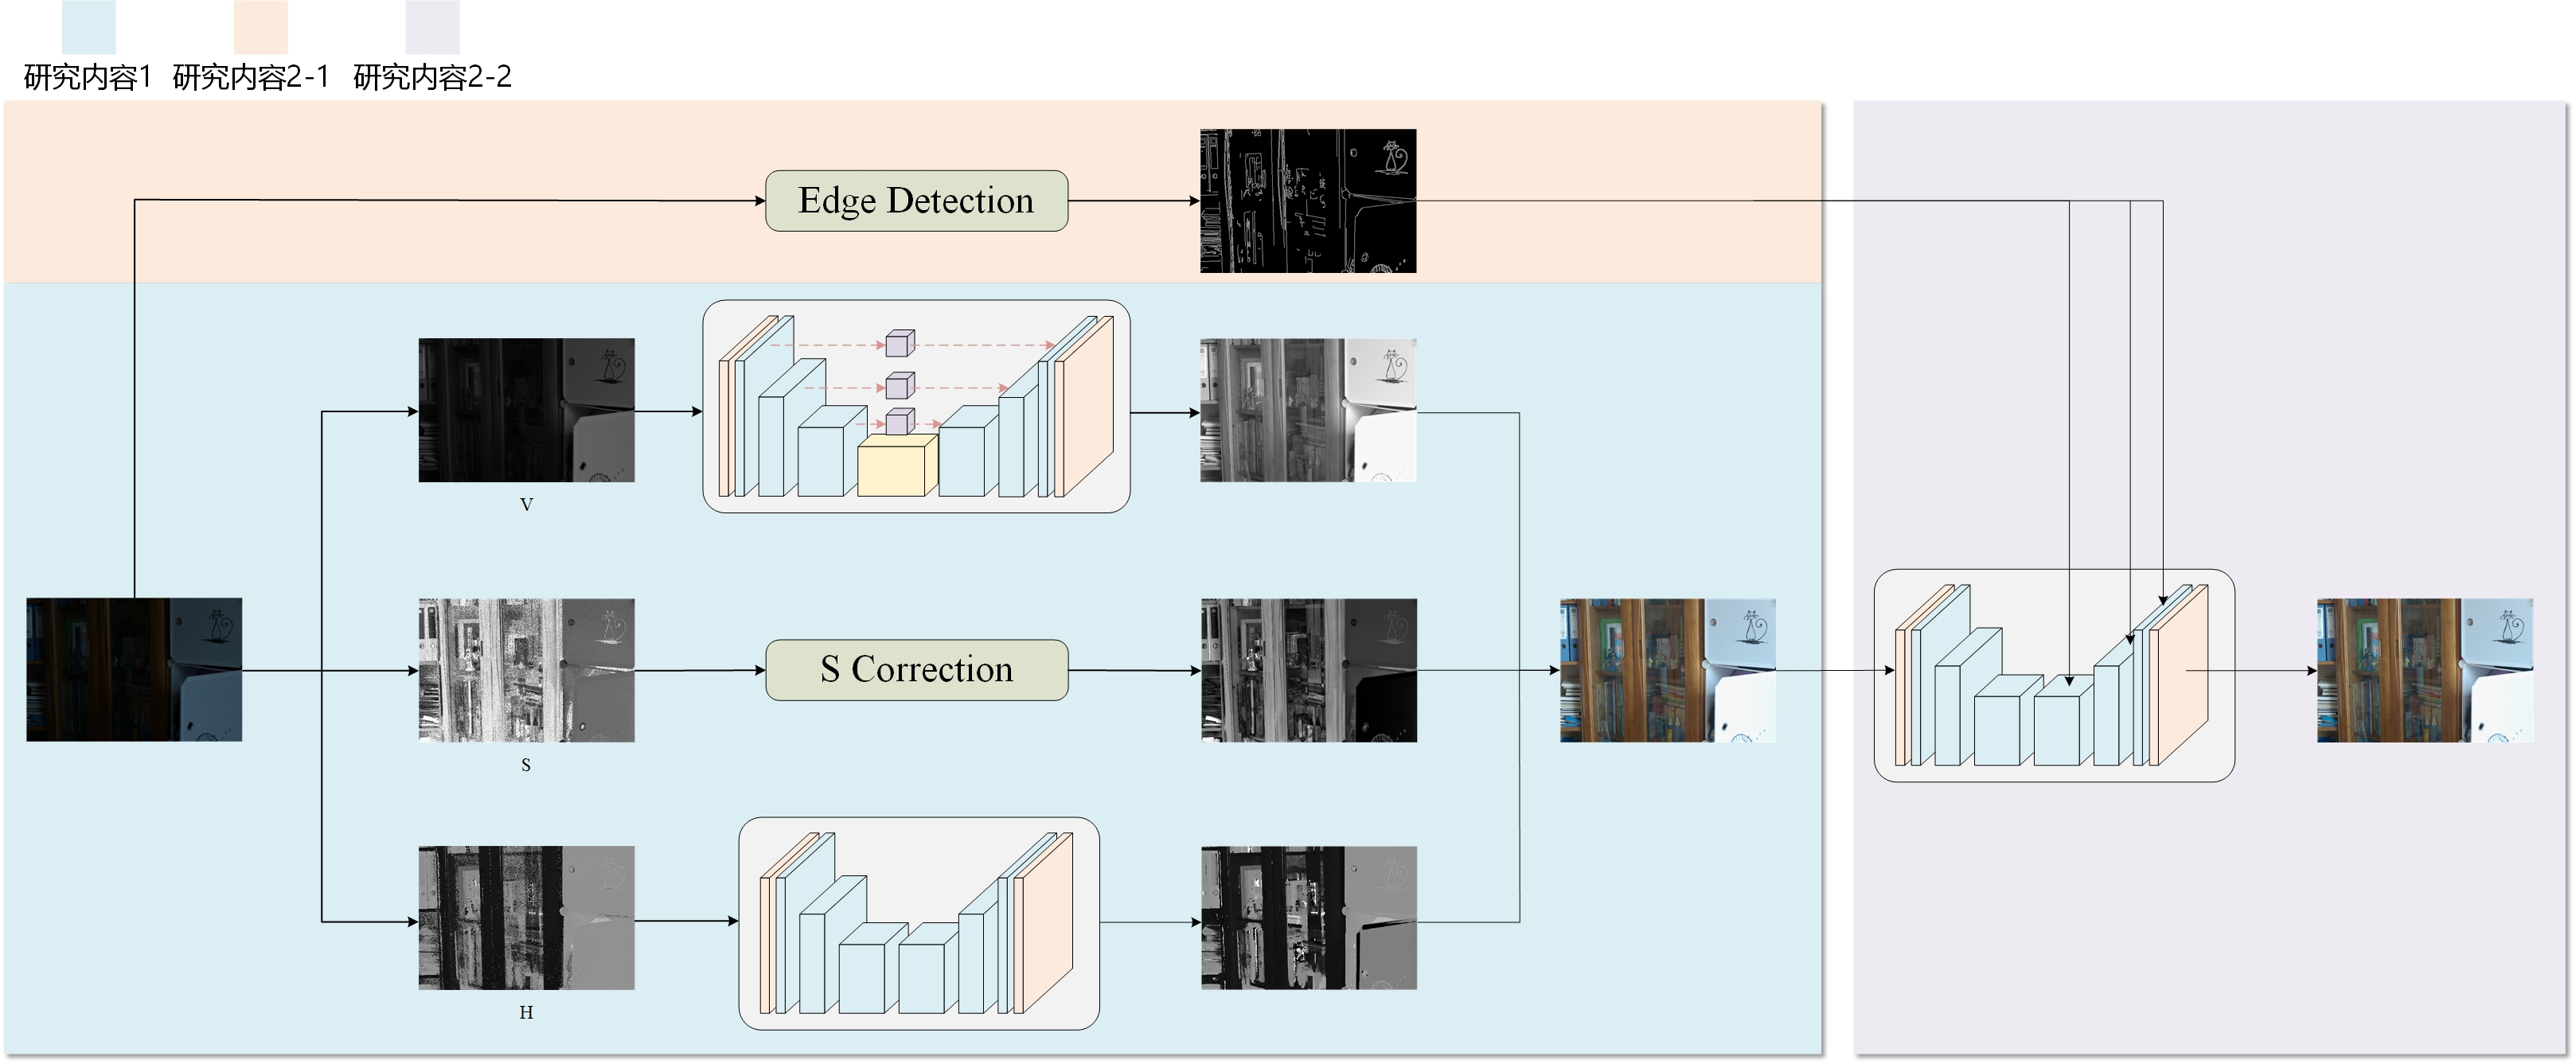
\includegraphics[width=\textwidth]{picture/LLIE/My Architecture/HSV Architecture}
			\end{center}
		\end{figure}
		
	\end{frame}
	
	\subsection{V通道增强模型}
	
	\begin{frame}
		\begin{figure}
			\centering			
			\begin{minipage}{.4\columnwidth}
				\setlength{\abovecaptionskip}{0.2cm}
				\centering
				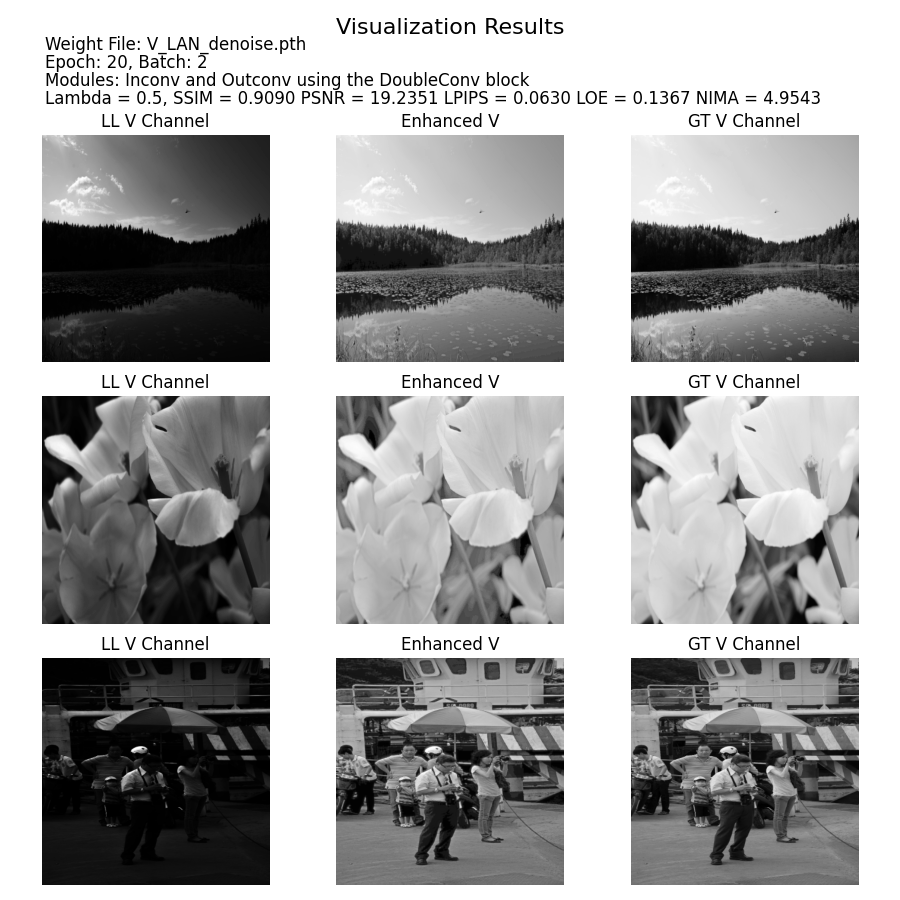
\includegraphics[width=\textwidth]{picture/LLIE/Experiment/myplot_V_LAN_denoise}
				\caption*{\tiny Visualization Results}
			\end{minipage}
			\begin{minipage}{.58\columnwidth}
				\setlength{\abovecaptionskip}{-0.05cm}
				\centering
				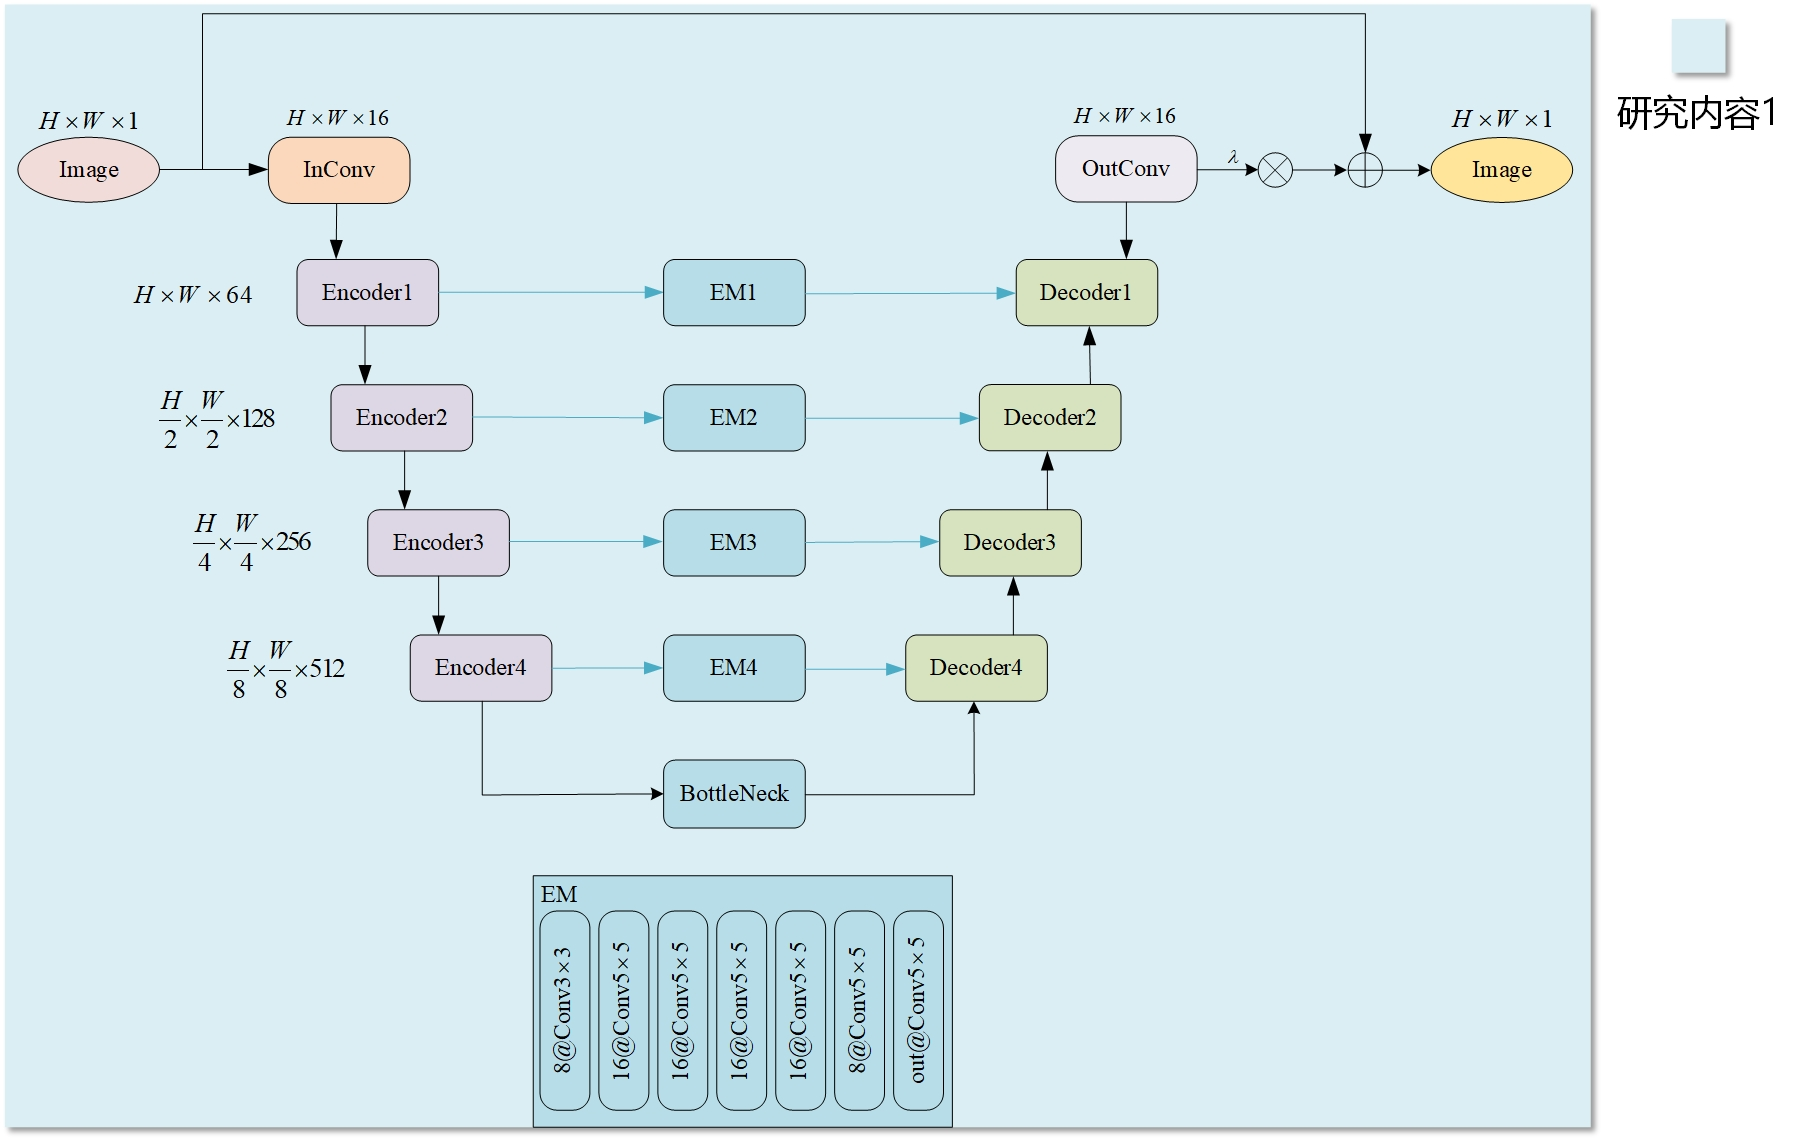
\includegraphics[width=\textwidth]{picture/LLIE/My Architecture/Baseline}
				%\caption{
					%	\label{fig: application scenarios}
					%	\tiny Application scenarios.
					%}
			\end{minipage}
		\end{figure}

	\end{frame}
	
%	\begin{frame}
%		\section{Literature Review}
%		Study hard and make progress every day. % 第一等级
%		\begin{itemize} 
%			\item Study hard and make progress every day. % 第二等级
%			\begin{itemize}
%				\item Study hard and make progress every day. % 第三等级
%				\begin{itemize}
%					\item Study hard and make progress every day. % 第四等级
%				\end{itemize}
%			\end{itemize}
%		\end{itemize}
%	\end{frame}
	
	\subsection{增强模型组件}
	
	\begin{frame}
	
		\begin{figure}
			\centering			
			\begin{minipage}{.45\columnwidth}
				\setlength{\abovecaptionskip}{0.2cm}
				\centering
				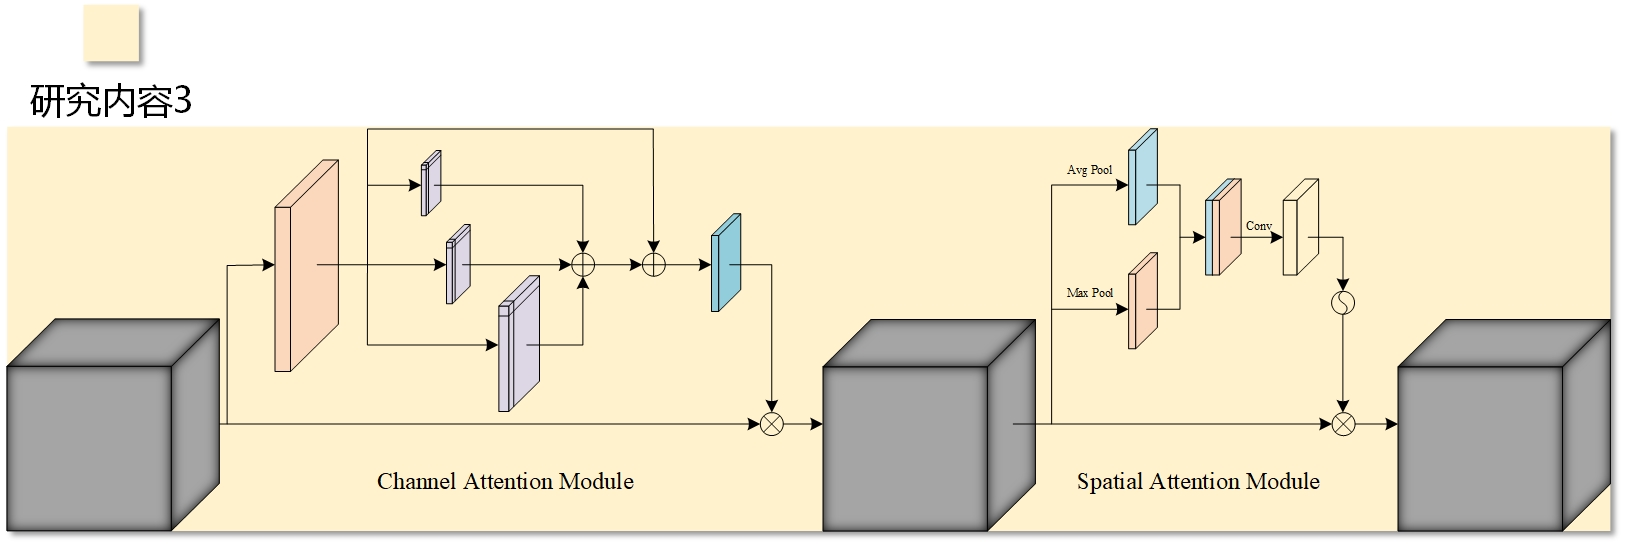
\includegraphics[width=\textwidth]{picture/LLIE/Experiment/Attention/MSAM}
				\caption*{\tiny MSAM Attention}
			\end{minipage}
			\begin{minipage}{.45\columnwidth}
				\setlength{\abovecaptionskip}{-0.05cm}
				\centering
				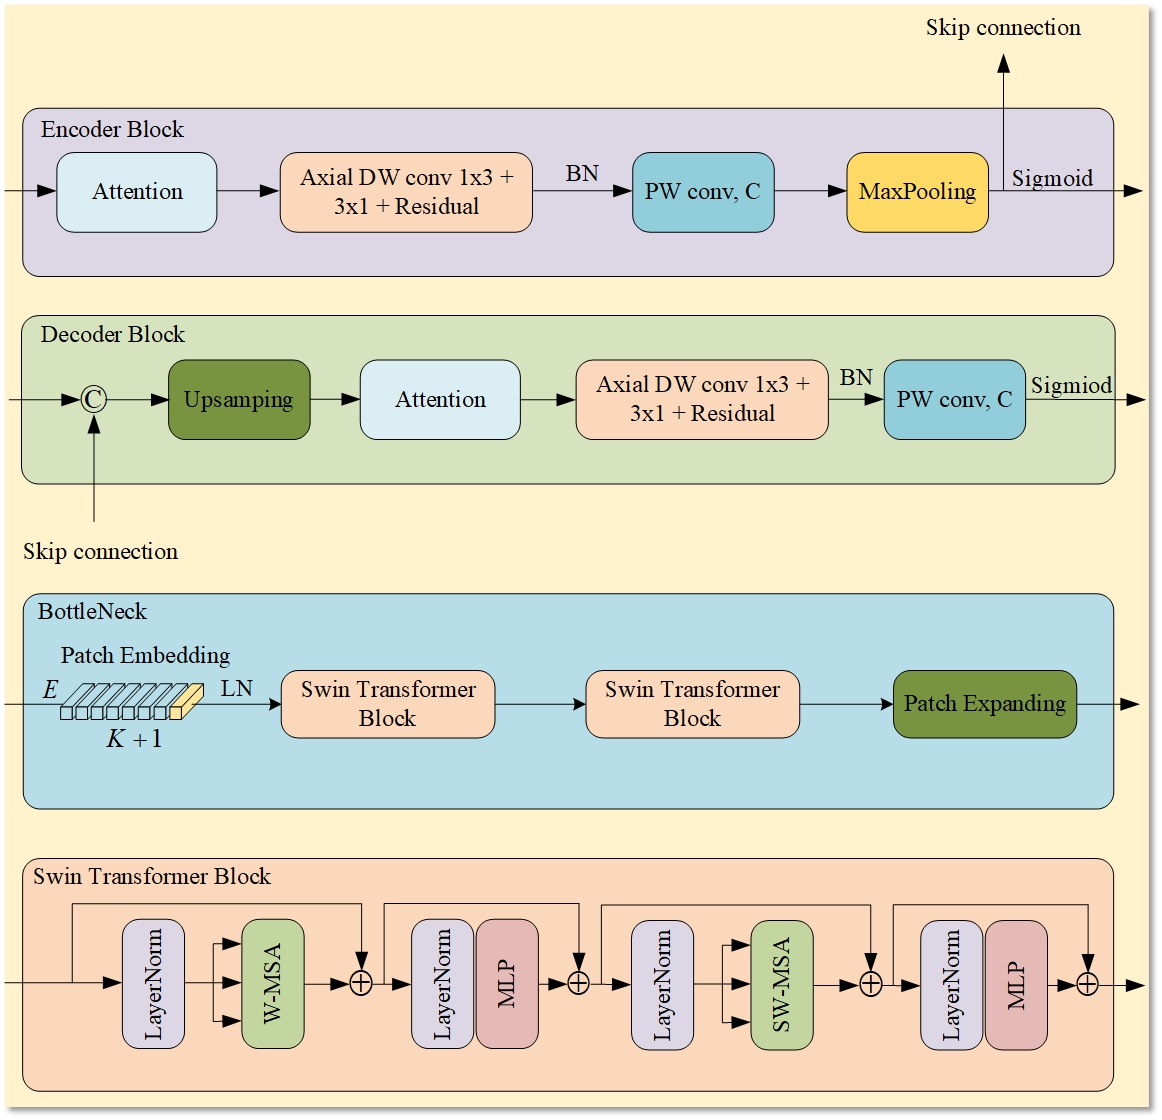
\includegraphics[width=\textwidth]{picture/LLIE/My Architecture/Encoder_Decoder}
				%\caption{
				%	\label{fig: application scenarios}
				%	\tiny Application scenarios.
				%}
			\end{minipage}
		\end{figure}
			
	\end{frame}
	
%	\begin{frame}
%		
%		\begin{figure}
%			\centering			
%			\begin{minipage}{.45\columnwidth}
%				\setlength{\abovecaptionskip}{0.2cm}
%				\centering
%				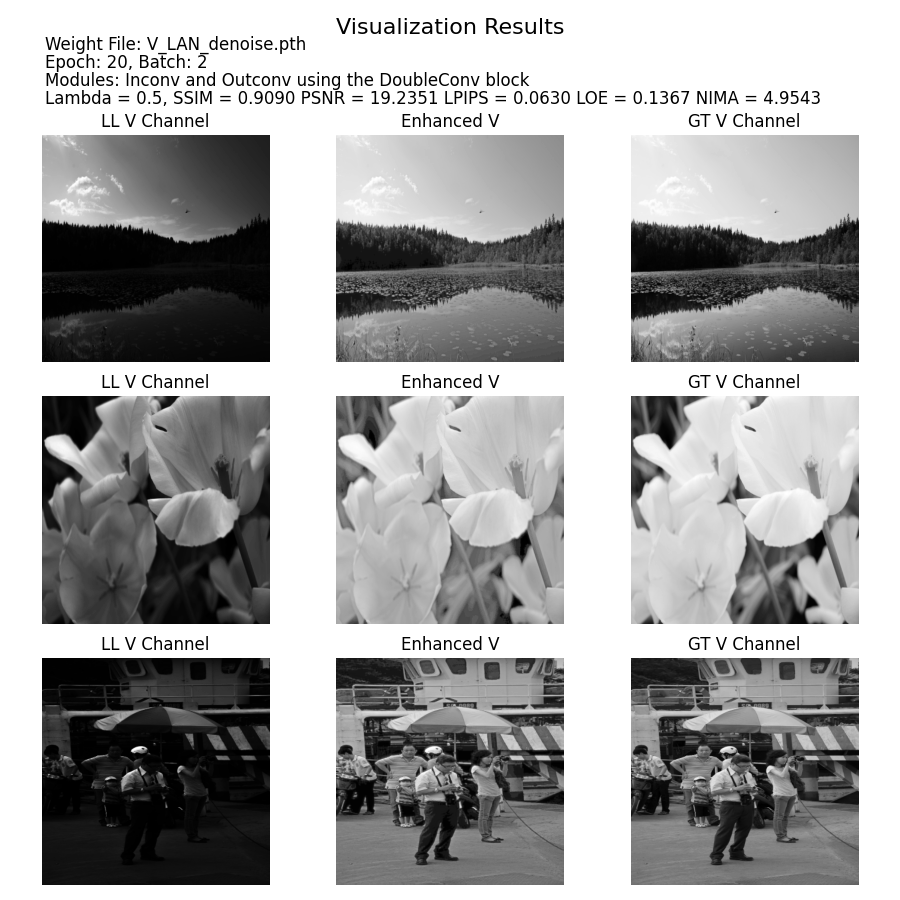
\includegraphics[width=\textwidth]{picture/LLIE/Experiment/myplot_V_LAN_denoise}
%				\caption*{\tiny Visualization Results}
%			\end{minipage}
%			\begin{minipage}{.45\columnwidth}
%				\setlength{\abovecaptionskip}{-0.05cm}
%				\centering
%				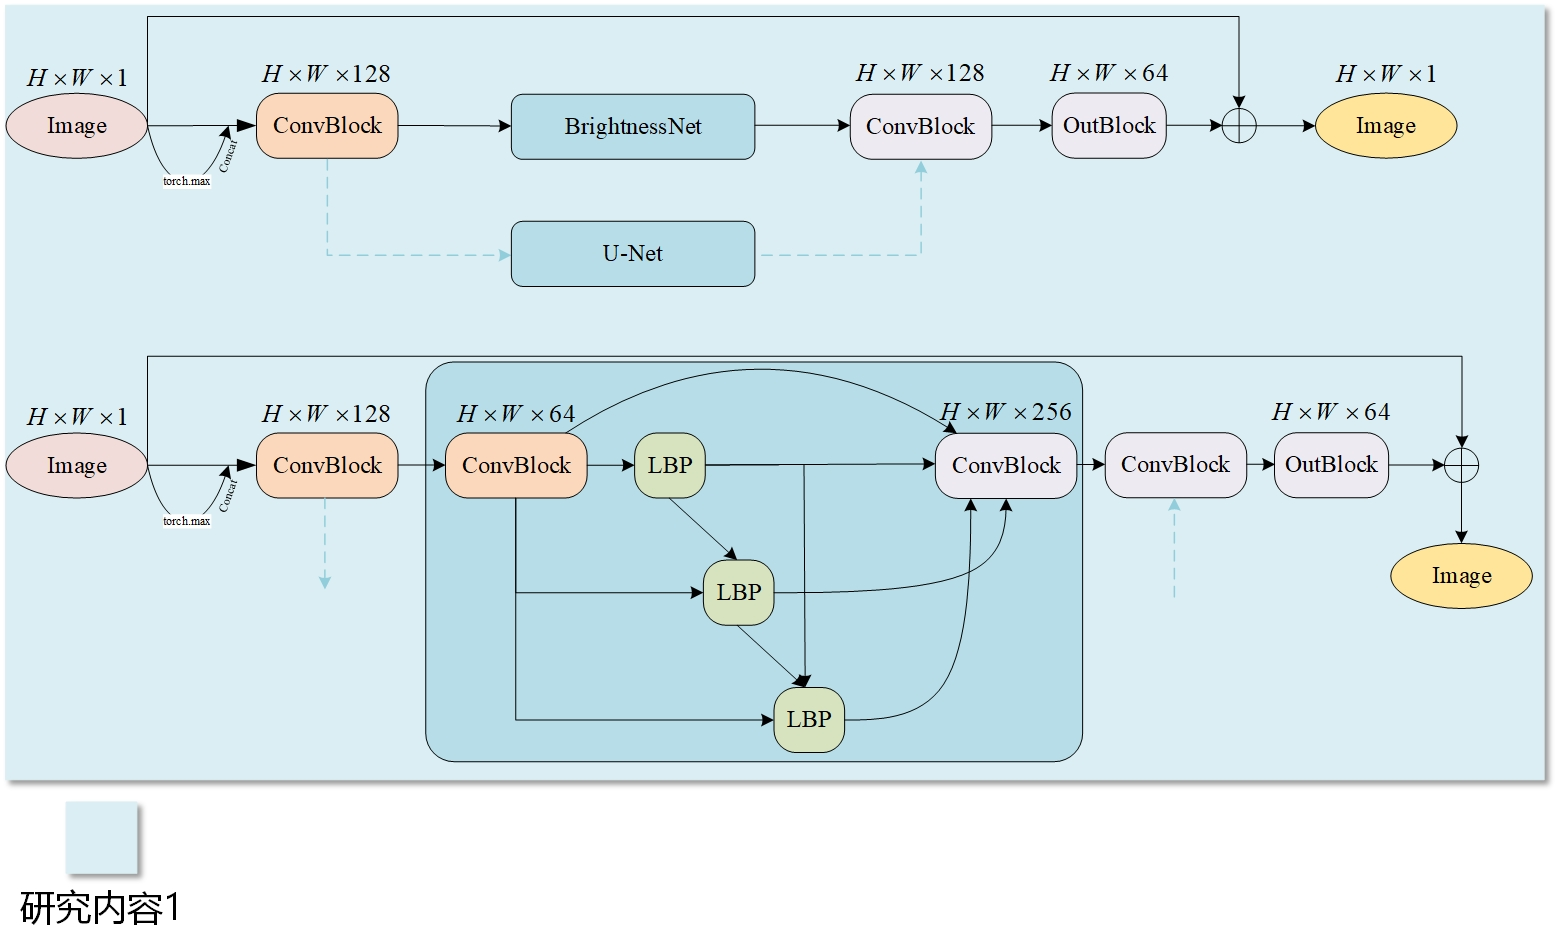
\includegraphics[width=\textwidth]{picture/LLIE/Experiment/UNet and LBP}
%				%\caption{
%					%	\label{fig: application scenarios}
%					%	\tiny Application scenarios.
%					%}
%			\end{minipage}
%		\end{figure}
%		
%	\end{frame}
	
	\subsection{边缘模型组件}
	
	\begin{frame}
		\begin{figure}
		\centering	
		\begin{minipage}{0.61\linewidth}
			\centering	
			\setlength{\abovecaptionskip}{-0.05cm}
			\begin{minipage}{0.16\textwidth}
				\includegraphics[width=\linewidth]{picture/Edge Detection/res(F-α)/Input/low00690} \\					
				\includegraphics[width=\linewidth]{picture/Edge Detection/res(F-α)/Input/low00692} \\
				\includegraphics[width=\linewidth]{picture/Edge Detection/res(F-α)/Input/low00694} \\
				\includegraphics[width=\linewidth]{picture/Edge Detection/res(F-α)/Input/low00696}
				\caption*{\tiny Input image}
			\end{minipage}
			\begin{minipage}{0.16\textwidth}
				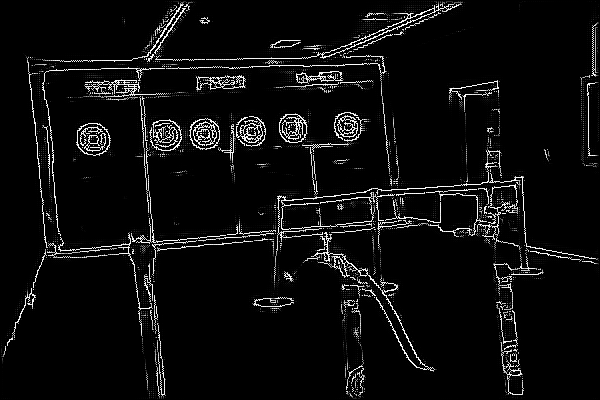
\includegraphics[width=\linewidth]{picture/Edge Detection/res(F-α)/GT/normal00690} \\
				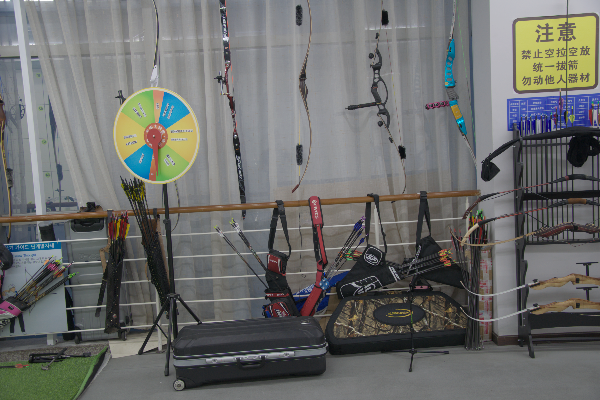
\includegraphics[width=\linewidth]{picture/Edge Detection/res(F-α)/GT/normal00692} \\
				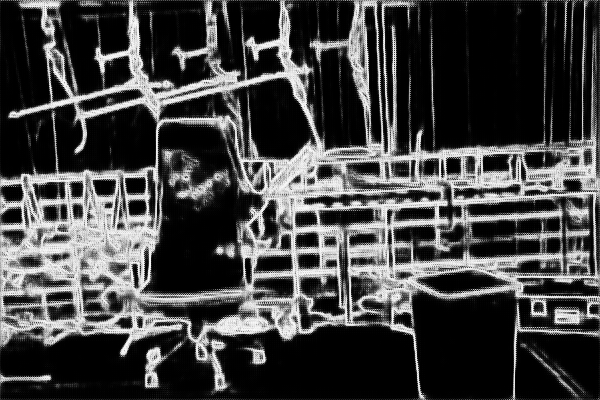
\includegraphics[width=\linewidth]{picture/Edge Detection/res(F-α)/GT/normal00694} \\
				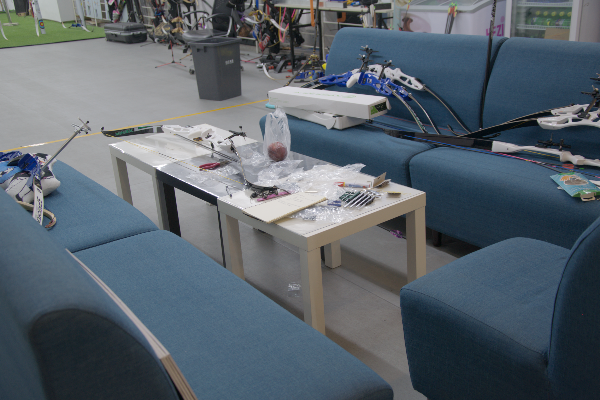
\includegraphics[width=\linewidth]{picture/Edge Detection/res(F-α)/GT/normal00696}
				\caption*{\tiny GT image}
			\end{minipage}
			\begin{minipage}{0.16\textwidth}
				\includegraphics[width=\linewidth]{picture/Edge Detection/res(F-α)/Predicted Edges/low00690} \\
				\includegraphics[width=\linewidth]{picture/Edge Detection/res(F-α)/Predicted Edges/low00692} \\
				\includegraphics[width=\linewidth]{picture/Edge Detection/res(F-α)/Predicted Edges/low00694} \\
				\includegraphics[width=\linewidth]{picture/Edge Detection/res(F-α)/Predicted Edges/low00696}
				\caption*{\tiny Pred Edges}
			\end{minipage}
			\begin{minipage}{0.16\textwidth}
				\includegraphics[width=\linewidth]{picture/Edge Detection/res(F-α)/Predicted Edges NMS/low00690} \\
				\includegraphics[width=\linewidth]{picture/Edge Detection/res(F-α)/Predicted Edges NMS/low00692} \\
				\includegraphics[width=\linewidth]{picture/Edge Detection/res(F-α)/Predicted Edges NMS/low00694} \\
				\includegraphics[width=\linewidth]{picture/Edge Detection/res(F-α)/Predicted Edges NMS/low00696}
				\caption*{\tiny Pred NMS}
			\end{minipage}
			\begin{minipage}{0.16\textwidth}
				\includegraphics[width=\linewidth]{picture/Edge Detection/res(F-α)/GT Edges/low00690} \\
				\includegraphics[width=\linewidth]{picture/Edge Detection/res(F-α)/GT Edges/low00692} \\
				\includegraphics[width=\linewidth]{picture/Edge Detection/res(F-α)/GT Edges/low00694} \\
				\includegraphics[width=\linewidth]{picture/Edge Detection/res(F-α)/GT Edges/low00696}
				\caption*{\tiny GT Edge}
			\end{minipage}
			\caption*{\tiny 基于 $\mathcal{D}^{low}_{2}$ 使用“低光-边缘”数据对,对 ${\left[\mathcal{F}\text{-}\alpha\right]}^{\mathcal{E}}_1$ 进行训练,对 $\mathcal{I}_{1 \sim 4}^{LL}$ 进行推理的可视化结果.}
		\end{minipage}	
		\begin{minipage}{0.38\linewidth}
			\begin{minipage}{\textwidth}
				\setlength{\abovecaptionskip}{-0.05cm}
				\centering
				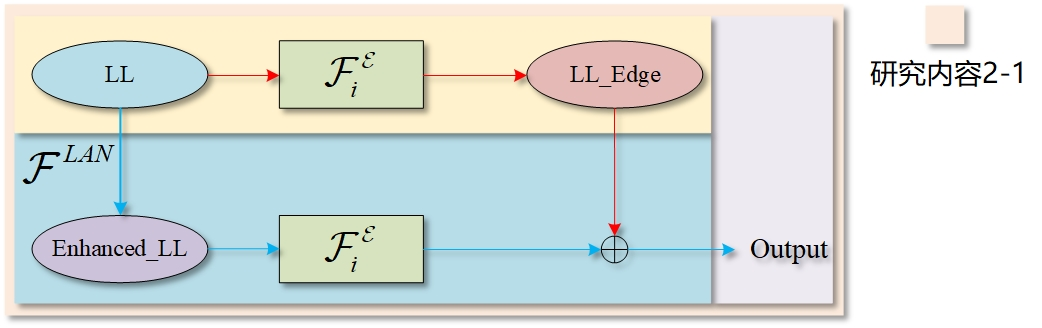
\includegraphics[width=\textwidth]{picture/Edge Detection/DCMP}
				\caption*{\tiny Edge detection network}
			\end{minipage}
			\begin{minipage}{\textwidth}
				\begin{table}[!htbp]
					\centering
					\tiny
					\resizebox{\textwidth}{!}{ %按照宽度调整调整表格大小
					\begin{tabular}{cccccc}		
						\hline
						\textbf{Branch} & \textbf{Dataset} & \textbf{ODS} & \textbf{OIS} & \textbf{AP} & \textbf{R50}  \\
						\hline
						${\left[\mathcal{F}\text{-}\alpha\right]}^{\mathcal{E}}_1$ & LOL-v2  & .863 & .888 & .915 & .997 \\
						${\left[\mathcal{F}\text{-}\alpha\right]}^{\mathcal{E}}_1$ & BIPED-v2& .807 & .813 & .871 & .942 \\
						${\left[\mathcal{F}\text{-}\beta\right]}^{\mathcal{E}}_1$  & LOL-v2  & .844 & .866 & .795 & .925 \\
						${\left[\mathcal{F}\text{-}\beta\right]}^{\mathcal{E}}_1$  & BIPED-v2& .759 & .767 & .800 & .861 \\
						${\left[\mathcal{F}\text{-}\gamma\right]}^{\mathcal{E}}_1$ & LOL-v2  & .863 & .888 & .915 & .997 \\
						${\left[\mathcal{F}\text{-}\gamma\right]}^{\mathcal{E}}_1$ & BIPED-v2& .807 & .813 & .871 & .942 \\
						\hline
					\end{tabular}
					}
					\captionsetup{font=scriptsize} %设置标题字体与表格字体一致
					\caption*{\tiny 不同的训练和推理方式的结果}		
				\end{table}
			\end{minipage}
		\end{minipage}	
		\end{figure}
		\end{frame}
	
	\section{后续计划}
	
	\subsection{模型的改进}
	
	\begin{frame}
		\begin{figure}
		\centering			
			\begin{minipage}{.45\columnwidth}
				\setlength{\abovecaptionskip}{-0.05cm}
				\centering
				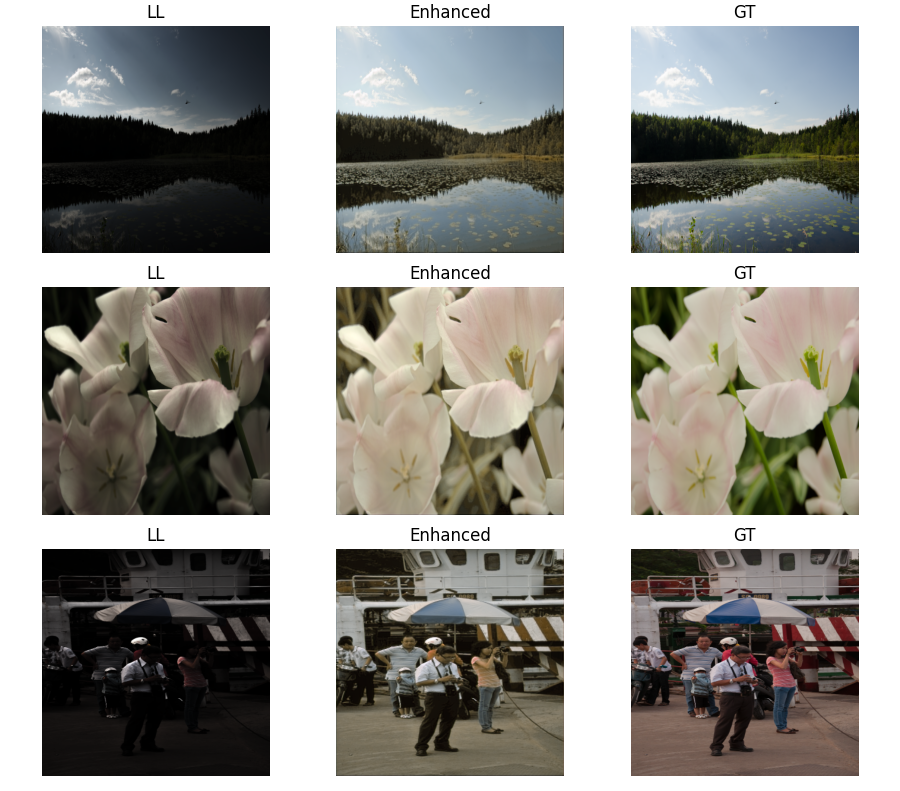
\includegraphics[width=\textwidth]{picture/LLIE/Experiment/myplot_LAN1}
				\caption*{
					\tiny HSV enhanced result. PSNR = 27.890 SSIM = 0.801
				}
			\end{minipage}
			\begin{minipage}{.47\columnwidth}
				\begin{itemize}
					\item \textbf{后续任务}
					
					\vspace{.3cm}
					
					\item[\checkmark] 
					\zihao{-6} \yahei 添加颜色相关的损失函数,通过实验设计更有效的损失函数搭配,并进一步改进 S 通道校正方法(研究内容1);
					
					% 论文提出了一种基于 GAN Loss 的模型去对结构信息建模,通过获得的结构信息指导增强。
					\vspace{.3cm}
					\item[\checkmark] 
					\zihao{-6} \yahei 提出一种更有效的 H 通道增强方法(研究内容1);
					
					% 从低光图像中很难提取到好的结构信息,但是论文中提出的方法提取到的结构信息会好很多,并且用于指导图像增强信息。
					
					\vspace{.3cm}
					\item[\checkmark] 
					\zihao{-6} \yahei 提出一种用于边缘指导低光图像增强的方法(研究内容2-2);
					
					\vspace{0.3cm}
					\item[\checkmark] 
					\zihao{-6} \yahei 将所提出的低光边缘提取模型和低光图像增强模型应用到具体的案例中;
					
					\vspace{0.3cm}
					\item[\checkmark] 
					\zihao{-6} \yahei 对模型进行轻量化设计。
				\end{itemize}	
			\end{minipage}
		\end{figure}
		
		
		
		
	\end{frame}
	
	\begin{frame}[plain,c]
		\begin{center}
			\Huge Thank you !
		\end{center}
	\end{frame}
	
%	\appendix
%	\begin{frame}[allowframebreaks]{References}
%		\tiny
%		%\bibliographystyle{unsrt}
%		\bibliographystyle{elsarticle-harv}
%		\bibliography{reference}
%		%\bibliographystyle{plainnat}
%	\end{frame}
	
\end{document}
